% anhang.tex
\chapter{Visualisierung der Krautfäule}
\label{anahnge}
\begin{figure}[h!]
	\centering
	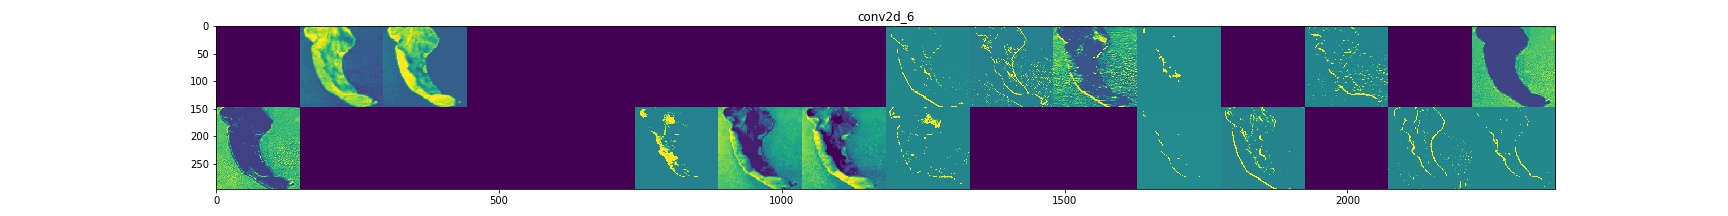
\includegraphics[width=\textwidth]{visualisierungen/late/activation/late_sample0.JPG}
	\caption{Visualisierung der Aktivierungswerte in der ersten Faltungschicht von der Krautfäule (eigene Darstellung).}
	\label{}
\end{figure}

\begin{figure}[h!]
	\centering
	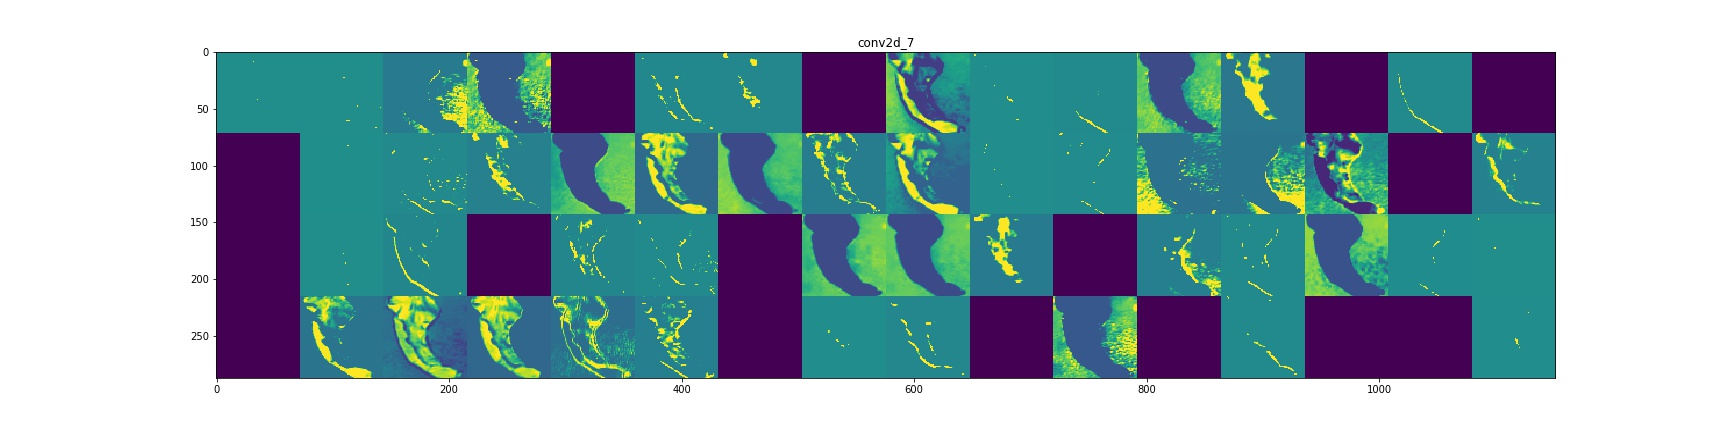
\includegraphics[width=\textwidth]{visualisierungen/late/activation/late_sample3.JPG}
	\caption{Visualisierung der Aktivierungswerte in der zweiten Faltungschicht von der Krautfäule (eigene Darstellung).}
	\label{}
\end{figure}

\begin{figure}[h!]
	\centering
	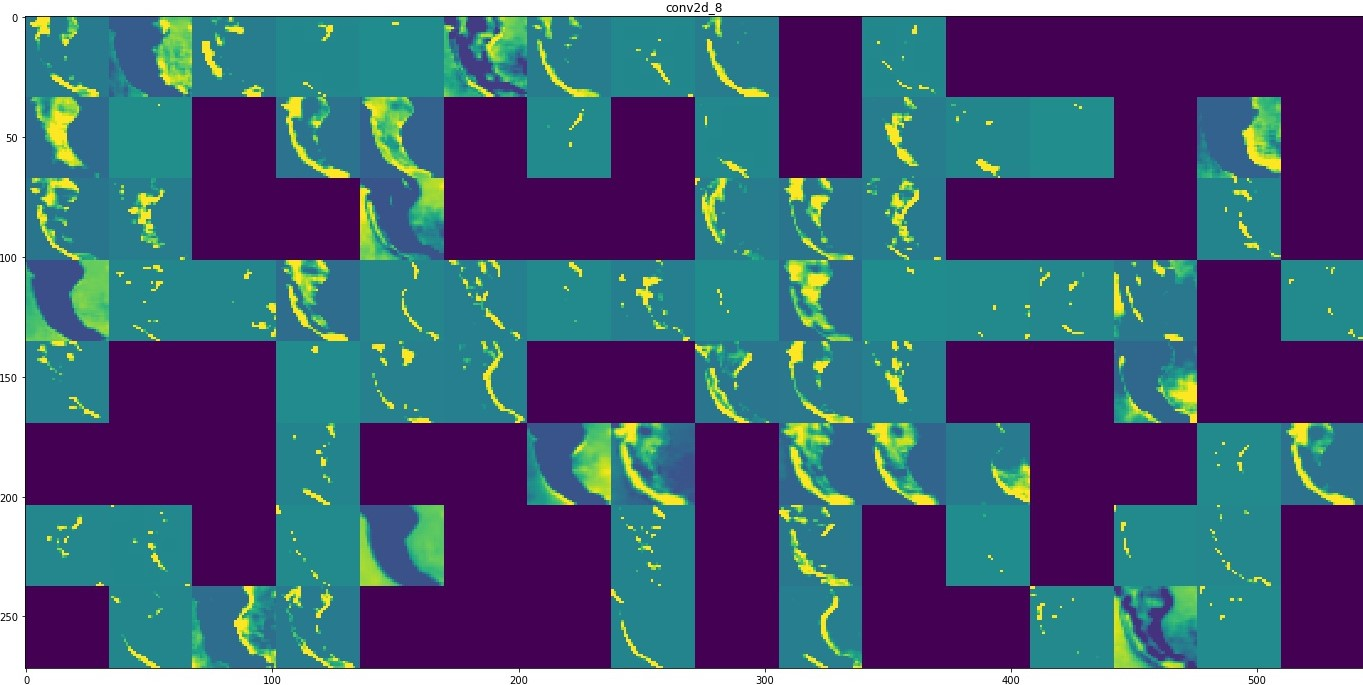
\includegraphics[width=\textwidth]{visualisierungen/late/activation/late_sample6.JPG}
	\caption{Visualisierung der Aktivierungswerte in der dritten Faltungschicht von der Krautfäule (eigene Darstellung).}
	\label{}
\end{figure}

\begin{figure}[h!]
	\centering
	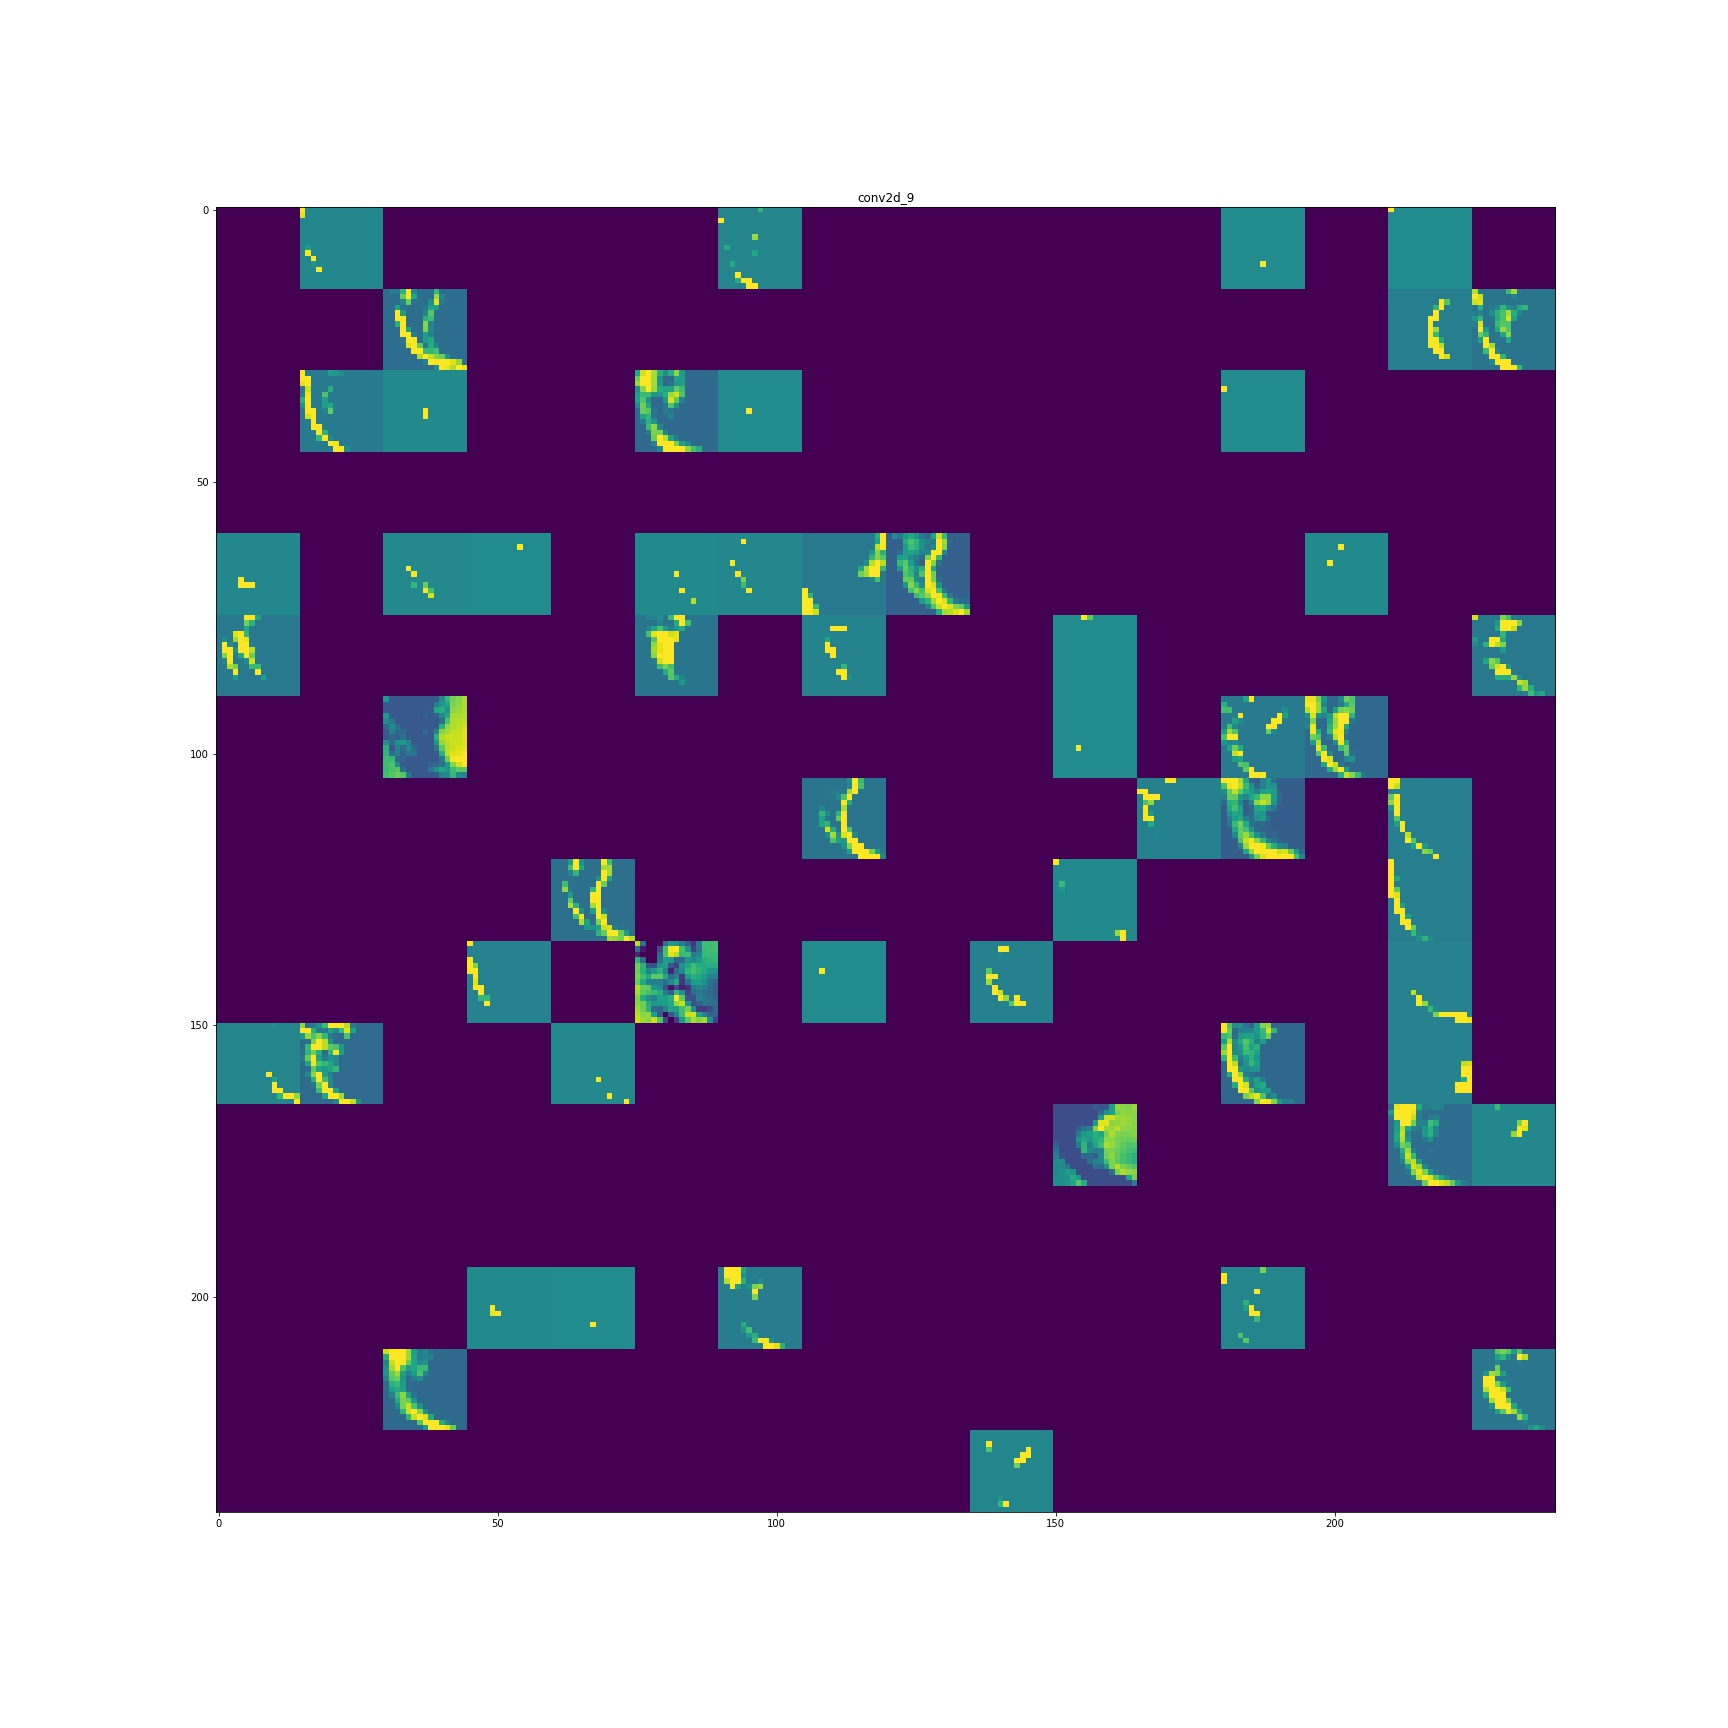
\includegraphics[width=\textwidth]{visualisierungen/late/activation/late_sample8.JPG}
	\caption{Visualisierung der Aktivierungswerte in der vierten Faltungschicht von der Krautfäule (eigene Darstellung).}
	\label{}
\end{figure}

\begin{figure}[h!]
	\centering
	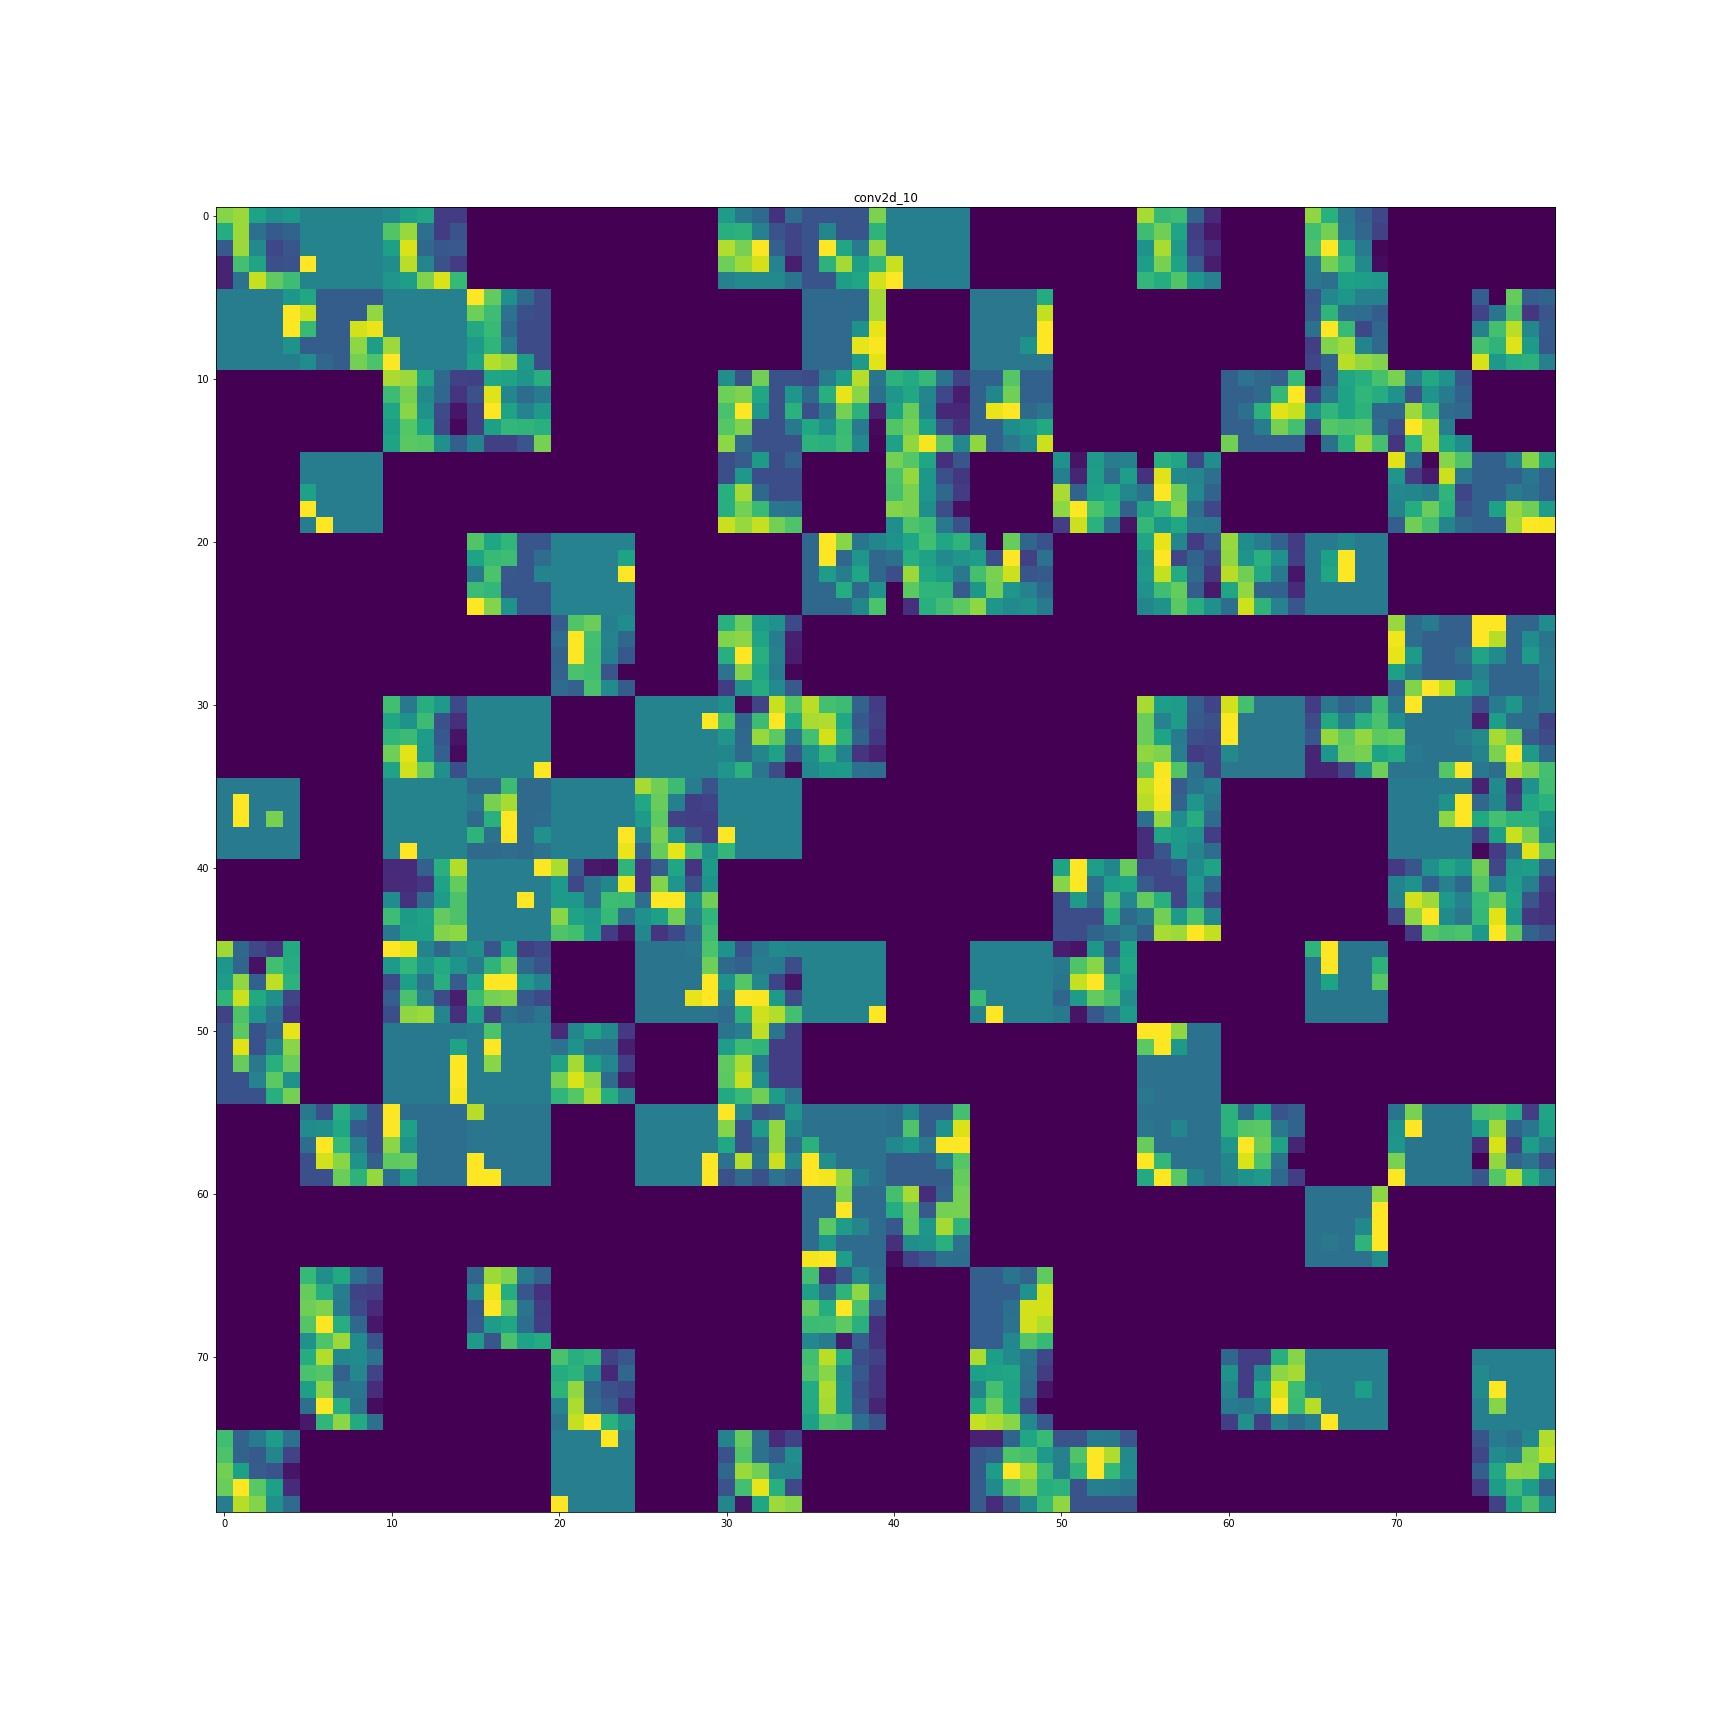
\includegraphics[width=\textwidth]{visualisierungen/late/activation/late_sample10.JPG}
	\caption{Visualisierung der Aktivierungswerte in der fünften Faltungschicht von der Krautfäule (eigene Darstellung).}
	\label{}
\end{figure}

%%%%%%%%%%%%%%%%%%%%%%%%%%%%%%%%%%%%%%%%%%%%%%

\begin{figure}[h!]
	\centering
	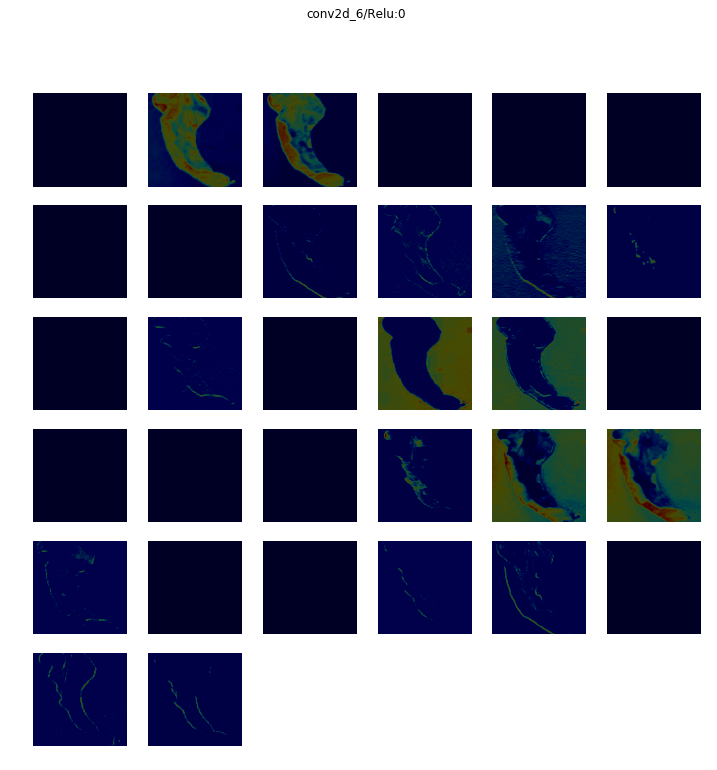
\includegraphics[width=\textwidth]{visualisierungen/late/heatmap_mit/conv2d_6.png}
	\caption{Visualisierung der Aktivierungswerte als Heatmap in der ersten Faltungschicht von der Krautfäule (eigene Darstellung).}
	\label{}
\end{figure}

\begin{figure}[h!]
	\centering
	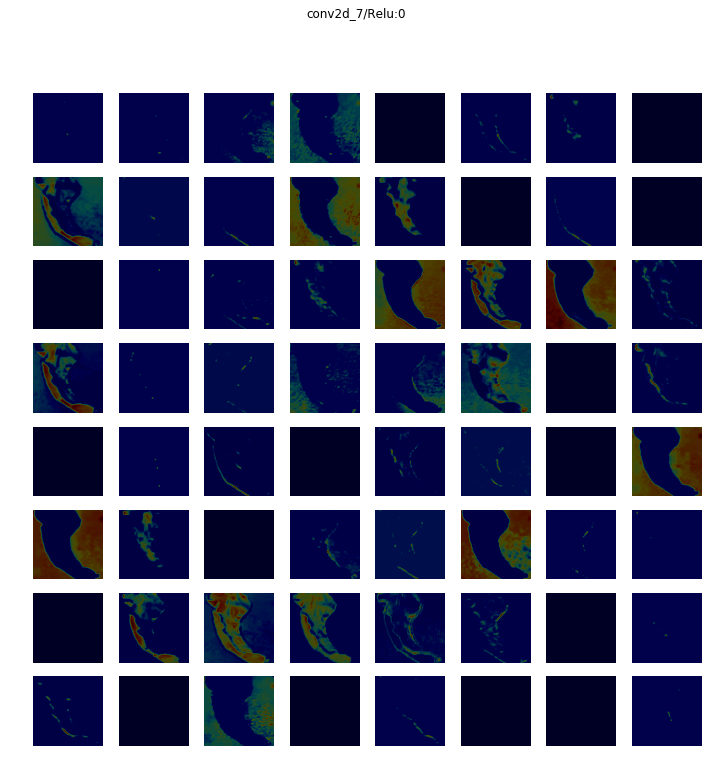
\includegraphics[width=\textwidth]{visualisierungen/late/heatmap_mit/conv2d_7.png}
	\caption{Visualisierung der Aktivierungswerte als Heatmap in der zweiten Faltungschicht von der Krautfäule (eigene Darstellung).}
	\label{}
\end{figure}

\begin{figure}[h!]
	\centering
	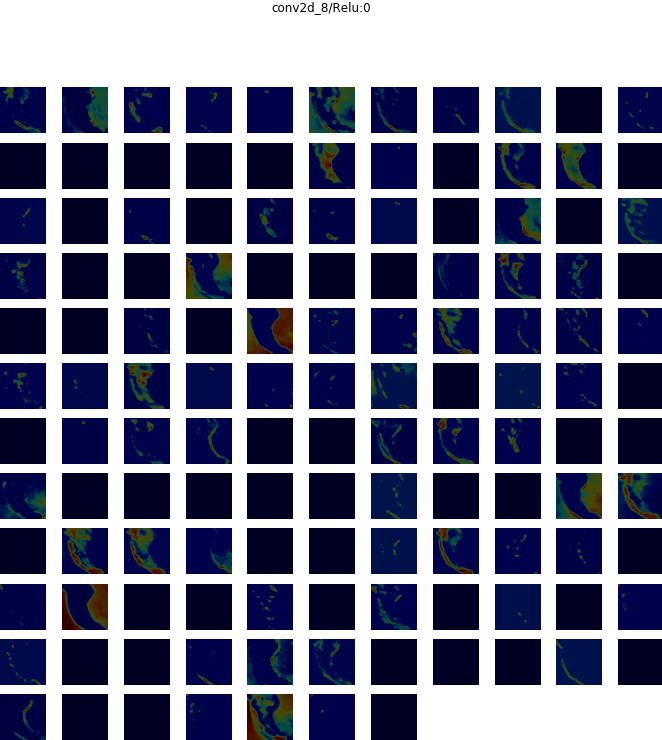
\includegraphics[width=\textwidth]{visualisierungen/late/heatmap_mit/conv2d_8.png}
	\caption{Visualisierung der Aktivierungswerte als Heatmap in der dritten Faltungschicht von der Krautfäule (eigene Darstellung).}
	\label{}
\end{figure}

\begin{figure}[h!]
	\centering
	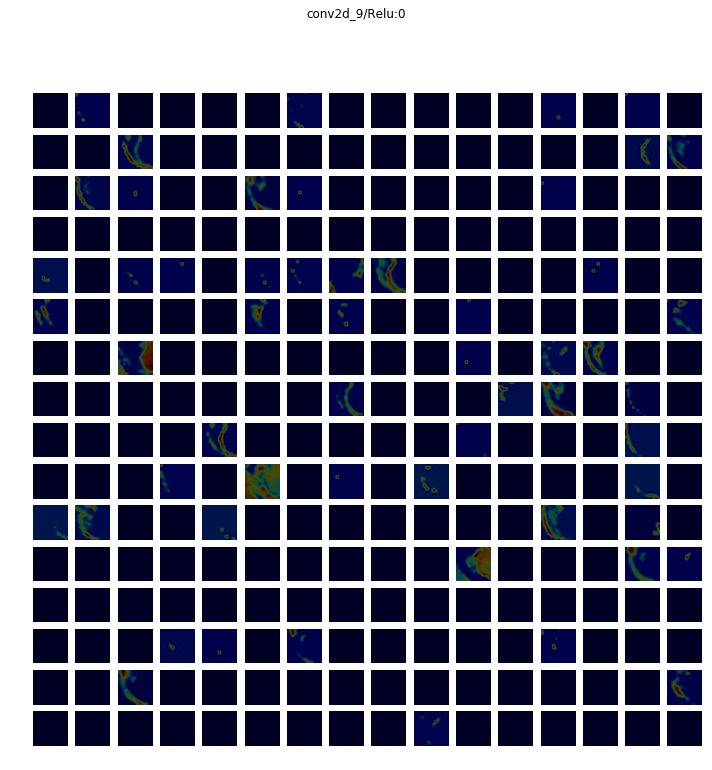
\includegraphics[width=\textwidth]{visualisierungen/late/heatmap_mit/conv2d_9.png}
	\caption{Visualisierung der Aktivierungswerte als Heatmap in der vierten Faltungschicht von der Krautfäule (eigene Darstellung).}
	\label{}
\end{figure}

\begin{figure}[h!]
	\centering
	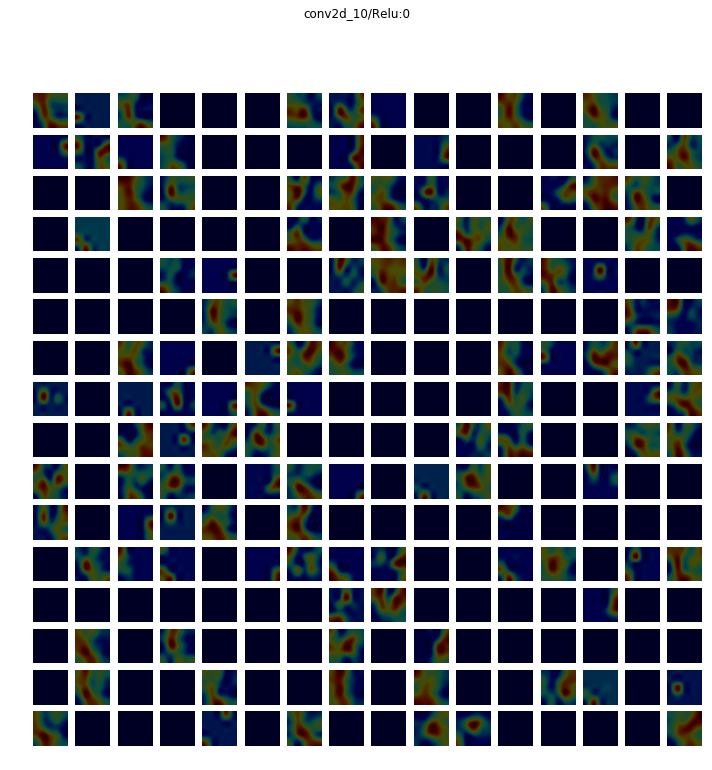
\includegraphics[width=\textwidth]{visualisierungen/late/heatmap_mit/conv2d_10.png}
	\caption{Visualisierung der Aktivierungswerte als Heatmap in der fünften Faltungschicht von der Krautfäule (eigene Darstellung).}
	\label{}
\end{figure}